\section{V1}
\subsection{Aufbau und Struktur der DNA}
\begin{itemize}
    \item[] \textbf{Purine}
    \item Adenin
    \item Guanin
\end{itemize}
\begin{itemize}
    \item[] \textbf{Pyrimidine}
    \item Thymin
    \item Cytosin
\end{itemize}

\subsection{Mitose}
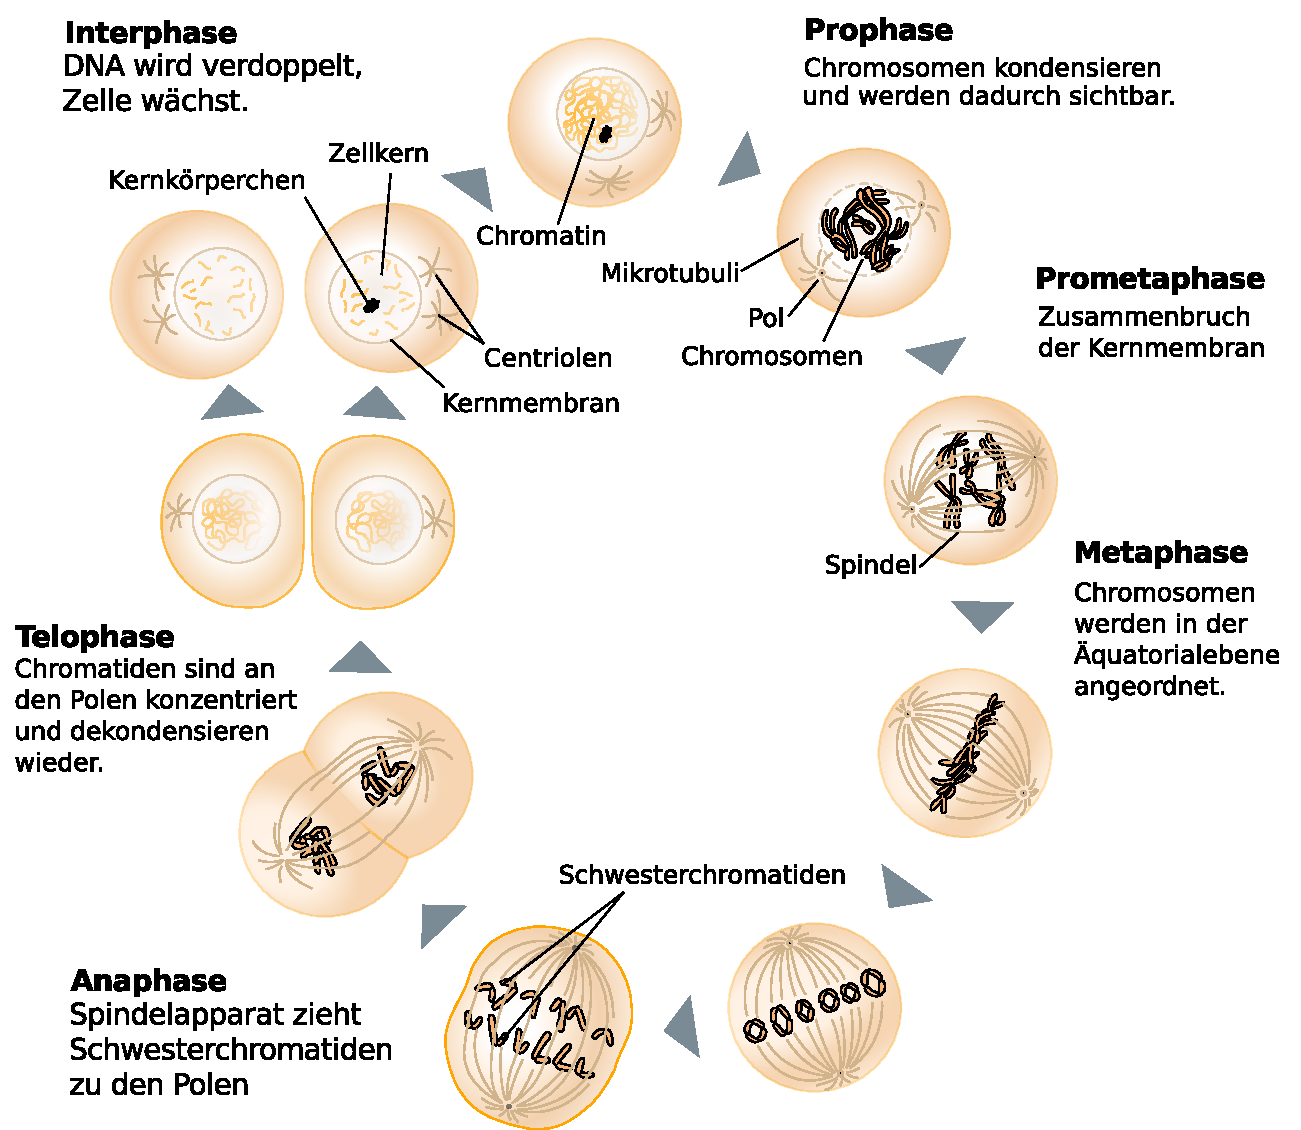
\includegraphics[width=1\textwidth]{lectures/V1/pix/Schemazeichnung_Mitose.pdf}\\
Zellzyklus mit Mitose\footnote{\url{https://de.wikipedia.org/wiki/Mitose}}

\subsection{Replikation, Transkription, Translation}

\subsubsection{Replikation}
\begin{itemize}
    \item Semikonservative Replikation (Meselson und Stahl, 1958) in drei Phasen:
        \begin{itemize}
            \item Initiation
            \item Elongation
            \item Terminierung
        \end{itemize}
    \item In der \textbf{Interphase} des Zellzyklus findet Replikation statt
    \item Der Vorgang der Kernteilung wird als \textbf{Mitose} bezeichnet
    \item DNA-Synthese nur in 5'$\rightarrow$3'-Richtung $\Rightarrow$ Folgestrang wird nicht-kontinuierlich synthetisiert $\Rightarrow$ Okazaki-Fragmente
\end{itemize}

\subsubsection{Transkription}
\begin{itemize}
    \item \textbf{Transkription} bezeichnet das ``Umschreiben'' der DNA in (m)RNA (Desoxyribonucleinsäure $\rightarrow$ Ribonucleinsäure; mit Thymin $\rightarrow$ Uracil)
    \item DNA-abhängige RNA-Polymerase synthetisiert RNA in 5'$\rightarrow$3'-Richtung
    \item Um Sense-Strang zu transkribieren, muss Antisense-Strang abgelesen werden (Sense-Strang $\underrightarrow{rev.-kompl.}$ Antisense-Strang $\underrightarrow{rev.-kompl.}$ mRNA = Sense-Strang)
    \item Splicing entfernt Introns, differentielles Splicing möglich $\Rightarrow$ verschiedene mögliche Genvarianten
    \item Transkription ist ein hochregulierter Prozess
\end{itemize}

\subsubsection{Translation}
\begin{itemize}
    \item \textbf{Translation} bezeichnet das ``Übersetzen'' der mRNA (Nucleinsäure, 4 Basen) in Protein (Peptid, ~20 Aminosäuren)
    \item Prozessierte mRNA verlässt den Zellkern und wird an Ribosomen Codon für Codon translatiert
    \item Ribosomen bestehen aus Protein und ribosomaler RNA
    \item tRNA ist der Adapter zwischen einem RNA-Anticodon, das komplementär auf die mRNA passt und einer Aminosäure
\end{itemize}

\subsection{Genetischer Code}
\begin{itemize}
    \item Der Genetische Code ist ein Triplett-Code, besteht also aus je drei aufeinanderfolgenden Basen-Tripletts, die für je eine Aminosäure codieren.
    \item Codierung häufiger Aminosäuren ist redundant, die dritte Stelle des Codes ist fast universell
\end{itemize}

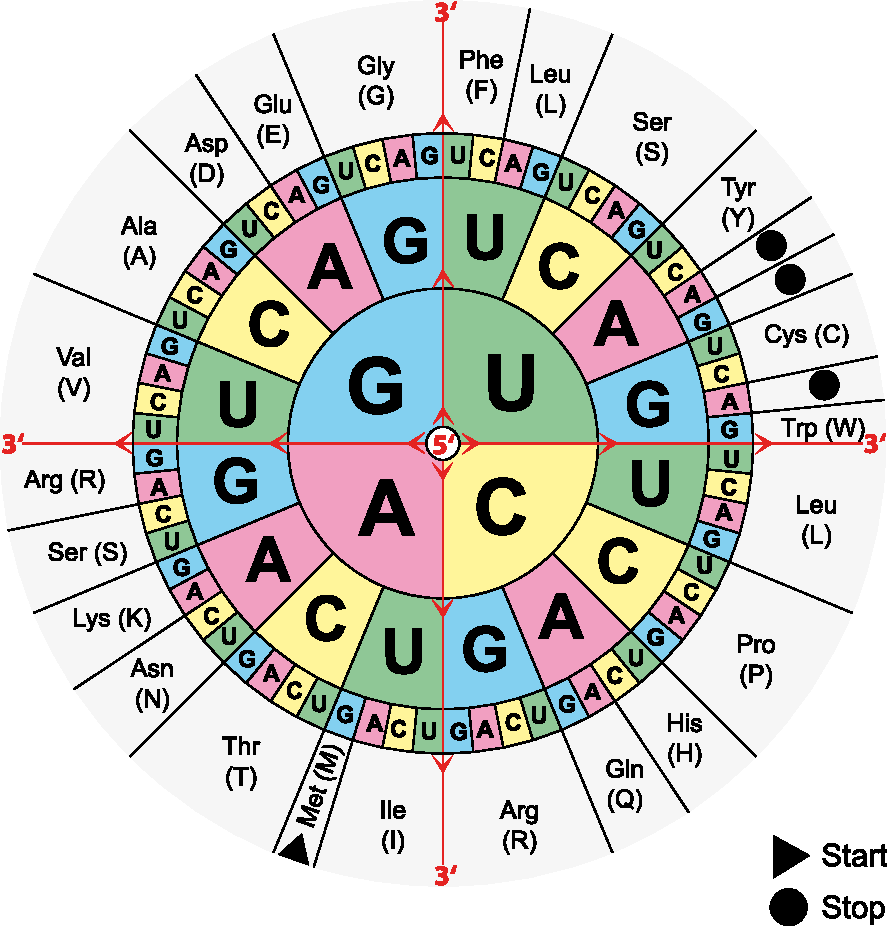
\includegraphics[width=1\textwidth]{lectures/V1/pix/Aminoacids_table.pdf}\\
``Codesonne''\footnote{\url{https://de.wikipedia.org/wiki/Genetischer_Code}}

\subsection{Nicht-kodierende RNAs}
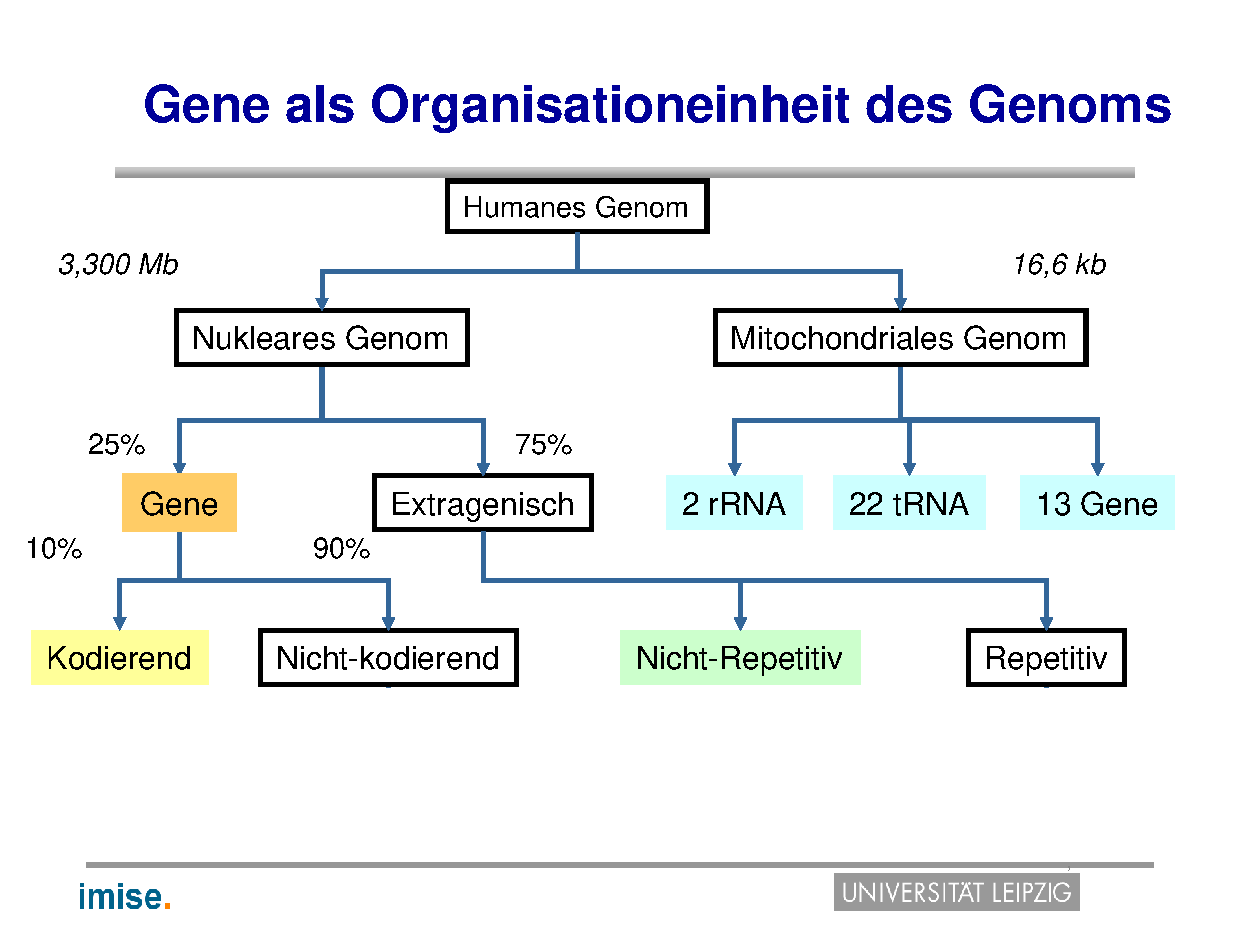
\includegraphics[width=1\textwidth]{lectures/V1/pix/31.pdf}\\
Humanes Genom (Scholz-VL)
\textbf{ncRNAs}
\begin{description}
    \item[microRNAs, siRNAs (ca. 18-25 nt)] Post-transkriptionales Gen-Silencing, RNA-Interferenz
    \item[Small RNAs (snoRNAs, smRNAs, piRNAs und andere; ca. 20-300 nt)] Modifizierung von targets-RNAs, Synthese von Telomer-DNA, Chromatinstruktur-Dynamik, Transkriptionsmodulation, Struktur, Gametogenese (?)
    \item[Medium und large RNAs (300-10000 nt oder mehr)] DNA-Imprinting, X-Inaktivierung, DNA-Demethylierung, Gentranskription, Herstellung anderer RNA-Klassen
\end{description}

\subsection{Aufgaben zur Übung 1}
\subsubsection{Aufgabe 1}

\begin{itemize}
	\item zu a: siehe Codonsonne\footnote{\url{https://de.wikipedia.org/wiki/Code-Sonne}}\\
		AUG (ATG) als Startcodon, UGA (TGA) als Stopcodon\\
		5' - ATG GTT AAA CAC GTG CAC GAG TGA - 3'\\
		3' - TAC CAA TTT GTG CAC GTG CTC ACT - 5'
	\item zu b:\\
		5' - AUG GUU AAA CAC GUG CAC GAG UGA - 3'
	\item zu c: tRNA für Valin, Lysin, Histidin, Valin, Glutamin, Glutaminsäure (das komplementäre der RNA)
	\item zu d: unpolar/neutral, positiv/basisch, positiv/basisch, unpolar/neutral, polar/neutral, negativ/sauer
	
\end{itemize}

\subsubsection{Aufgabe 2}

\subsubsection{Aufgabe 3}

\begin{itemize}
	\item E. coli: $4,6*10^6$ Basen, 4500 Gene
	\item Bäckerhefe: $2*10^7$ Basen, 6000 Gene
	\item Ackerschmalwand: $10^8$ Basen, 25500 Gene
	\item Fruchtfliege (Drosophila Melanogaster): $2*10^8$ Basen, 13500 Gene
	\item Menschen: $3,27 * 10^9$ Basen, 23000 Gene
\end{itemize}

\subsubsection{Aufgabe 4}

\begin{itemize}
	\item SNP\footnote{\url{https://de.wikipedia.org/wiki/Einzelnukleotid-Polymorphismus}}:
	\begin{itemize}
		\item Single Nucleotide Polymorphism - Einzelnukleotid-Polymorphismus
		\item Variation eines einzelnen Basenpaares in einem DNA-Strang
		\item SNPs sind geerbte und vererbbare genetische Varianten. Begrifflich davon abzugrenzen ist der Begriff der Mutation, der in der Regel eine neu aufgetretene Veränderung bezeichnet
		\item Laktosetoleranz: durch einen SNP im Intron des Gens mcm6 entwickelt, welches 5' von LCT(Lactase) liegt
	\end{itemize}
	\item CNV\footnote{\url{https://de.wikipedia.org/wiki/Gene_copy_number_variants}}:
	\begin{itemize}
		\item Copy number variation - Kopienzahlvariation
		\item struktureller Variation des Erbguts, die Abweichungen der Anzahl der Kopien eines bestimmten DNA-Abschnittes innerhalb eines Genoms erzeugt
	\end{itemize}
	\item Chromosomen-Mutationen\footnote{\url{https://de.wikipedia.org/wiki/Chromosomenmutation}}:
	\begin{itemize}
		\item strukturelle Veränderung eines Chromosoms, 5 Arten
		\item Deletion: Ein Teilstück des Chromosoms (Endstück oder mittlerer Abschnitt) geht verloren
    	\item Translokation: Chromosomen können auseinanderbrechen und dabei Teilstücke verlieren, welche in die Chromatide eines anderen Chromosoms angeheftet werden
	    \item Duplikation: Ein Abschnitt des Chromosoms ist doppelt vorhanden, da ein auseinandergebrochenes Teilstück in die Schwesterchromatide eingegliedert wurde
	    \item Inversion: Innerhalb eines Chromosoms kann sich nach einem doppelten Bruch ein Stück wieder umgekehrt einfügen
	    \item Insertion (auch: Addition): Hier besitzt ein Chromosom ein zusätzliches Teilstück
	\end{itemize}
\end{itemize}

\subsubsection{Aufgabe 5}
\begin{itemize}
	\item PCR\footnote{\url{https://de.wikipedia.org/wiki/Polymerase-Kettenreaktion}}: Polymerase-Kettenreaktion (polymerase chain reaction)
	\item Prozess besteht aus etwa 20–50 Zyklen, jeder Zyklus besteht aus drei Schritten
	\begin{enumerate}
		\item Denaturierung (Melting, Schmelzen): Zunächst wird die doppelsträngige DNA auf 94–96 $^\circ$C erhitzt, um die Stränge zu trennen. Die Wasserstoffbrückenbindungen, die die beiden DNA-Stränge zusammenhalten, werden aufgebrochen. Im ersten Zyklus wird die DNA oft für längere Zeit erhitzt (Initialisierung), um sicherzustellen, dass sich sowohl die Ausgangs-DNA als auch die Primer vollständig voneinander getrennt haben und nur noch Einzelstränge vorliegen. Manche (sogenannte Hot-Start-) Polymerasen müssen durch eine noch längere anfängliche Erhitzungsphase (bis zu 15 Minuten) aktiviert werden. Danach wird schnell auf 65 $^\circ$C abgekühlt, um die Rückbildung der Doppelhelix zu verhindern.
		\item Primerhybridisierung (primer annealing): Die Temperatur wird ca. 30 Sekunden lang auf einem Wert gehalten, der eine spezifische Anlagerung der Primer an die DNA erlaubt. Die genaue Temperatur wird hierbei durch die Länge und die Sequenz der Primer bestimmt (bzw. der passenden Nukleotide im Primer, wenn durch diesen Mutationen eingeführt werden sollen = site-directed mutagenesis). Wird die Temperatur zu niedrig gewählt, können sich die Primer unter Umständen auch an nicht hundertprozentig komplementären Sequenzen anlagern und so zu unspezifischen Produkten („Geisterbanden“) führen. Wird die Temperatur zu hoch gewählt, ist die thermische Bewegung der Primer u. U. so groß, dass sie sich nicht richtig anheften können, so dass es zu gar keiner oder nur ineffizienter Produktbildung kommt. Die Temperatur, welche die beiden oben genannten Effekte weitgehend ausschließt, liegt normalerweise 5–10 $^\circ$C unter dem Schmelzpunkt der Primersequenzen; dies entspricht meist einer Temperatur von 55 bis 65 $^\circ$C.
		\item Elongation (Extending, Polymerisation, Verlängerung, Amplifikation): Schließlich füllt die DNA-Polymerase die fehlenden Stränge mit freien Nukleotiden auf. Sie beginnt am 3'-Ende des angelagerten Primers und folgt dann dem DNA-Strang. Der Primer wird nicht wieder abgelöst, er bildet den Anfang des neuen Einzelstrangs. Die Temperatur hängt vom Arbeitsoptimum der verwendeten DNA-Polymerase ab (68–72 $^\circ$C). Dieser Schritt dauert etwa 30 Sekunden je 500 Basenpaare, variiert aber in Abhängigkeit von der verwendeten DNA-Polymerase. Übliche Thermocycler kühlen die Reaktionsansätze nach Vollendung aller Zyklen auf 4–8 $^\circ$C, so dass eine PCR am Abend angesetzt werden kann und die Proben am Morgen darauf weiterverarbeitet werden können.
	\end{enumerate}
\end{itemize}

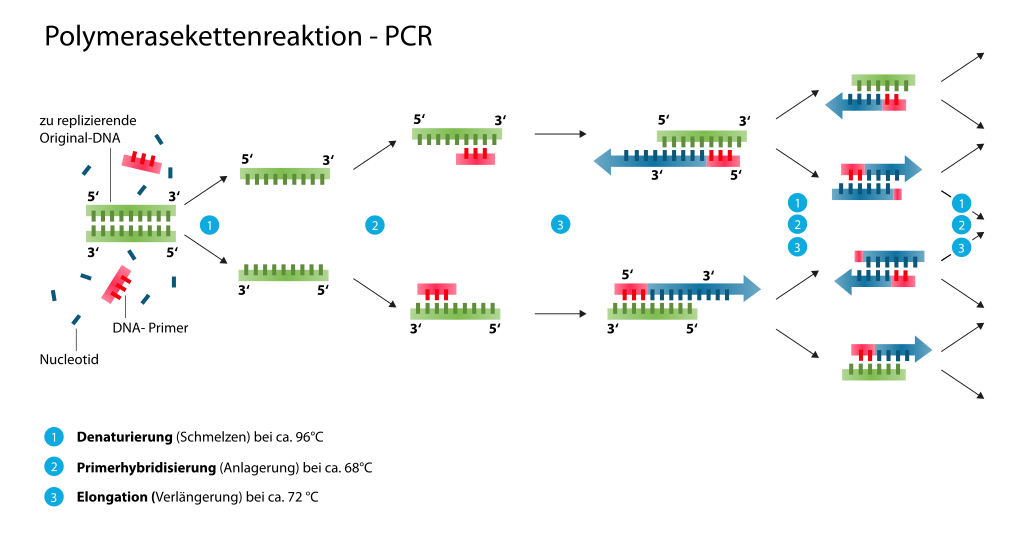
\includegraphics[width=1\textwidth]{lectures/V1/pix/1024px-Polymerasekettenreaktion.png}

zu amplifizierende Sequenz:\\
5‘ACCGCGGCTT AGGAAAXXXX XXXXXXCCCG GGGCGTATGC TGACGG3‘\\
\noindent\hspace*{17mm}3'-CGAA TCCTTT-5'\hspace*{23mm}3'-GGGC CCCGCA-5'

\subsubsection{Aufgabe 6}
Didesoxymethode nach Sanger\footnote{\url{https://de.wikipedia.org/wiki/DNA-Sequenzierung\#Didesoxymethode_nach_Sanger}}:
\begin{itemize}
	\item Didesoxynukleotide weil: wird als Stopp-Nukleotiden benutzt, an Ribose (Zucker) an Position 2' und 3' desoxidiert ist. Dadurch fehlt am 3'-Kohlenstoff-Atom die Hydroxygruppe, an der bei der Polymerisation das nächste Nukleotid angehängt wird.
	\item auch Desoxynukleotide weil: sonst funktioniert die Verlängerung nicht
	\item Ergebnis nur Didesoxynukleotide: es gibt keine Verländerung
\end{itemize}
nur Didesoxynukleotide
